\documentclass[a4paper,15pt]{exam}
\usepackage{kotex}
\usepackage{geometry}
\usepackage{amsmath}
\usepackage{tikz}
\usetikzlibrary{positioning}
\usepackage{scalerel,amssymb}
\usepackage{calc}
\usepackage{pst-3dplot}
\geometry{margin=0.5cm}

\begin{document}

\begin{center}
  \bfseries\LARGE

  수학 \#8
  \bigskip
  \normalfont\normalsize
\end{center}


\begin{questions}
\question
    $x$는 어떤 값입니까?
    \begin{parts}
        \part 
            $ 6 \times 3 = x + x + x $
            \answerline
        \part 
            $ 7 \times 6 = ( 7 \times 1 ) + ( 7 \times x ) $
            \answerline
        \part 
            $ 7 \times 6 = 14 + ( 7 \times x ) $
            \answerline
        \part 
            $ 7 \times 6 = 28 + ( 7 \times x ) $
            \answerline
    \end{parts}
\vspace{\stretch{1}}

\question
    사과가 한 상자에 9개씩, 배가 한 상자에 6개씩 들어 있습니다. 사과 3상자와 배 4상자에 들어 있는 과일은 모두 몇 개일까요?
\vspace{\stretch{1}}



\question
아래와 같이 상자가 쌓여 있다고 하자. 쌓인 상자의 수는 몇개인가?

    \begin{center}
        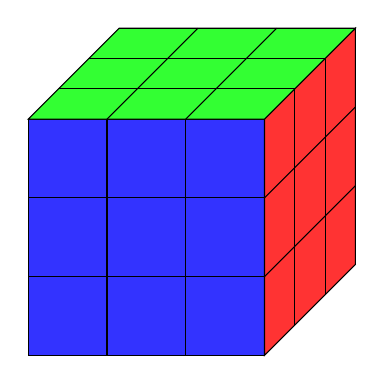
\begin{tikzpicture}
        \draw[fill=blue!80] (0,0,3)--(3,0,3)--(3,3,3)--(0,3,3)--cycle;
        \draw[fill=red!80] (3,0,0) -- (3,3,0)--(3,3,3)--(3,0,3)--cycle;
        \draw[fill=green!80] (3,3,0) -- (3,3,3)--(0,3,3)--(0,3,0)--cycle;
        \foreach \x in {1,2}
         {
        \draw(3,0,\x)--(3,3,\x); 
        \draw(3,\x,0)--(3,\x,3); 
        \draw(0,\x,3)--(3,\x,3); 
        \draw(\x,0,3)--(\x,3,3); 
        \draw(\x,3,0)--(\x,3,3); 
        \draw(0,3,\x)--(3,3,\x); 
        }
        \end{tikzpicture}
    \end{center}

\vspace{\stretch{1}}



\question
$6\times6$ 을 구하는 방법 3가지를 적고 가장 쉬운 방법은 무엇인지 말해보시오.
\vspace{\stretch{1}}


\question
$1 + 2 + 3 + 4 + 5 + 6 + 7 + 8 + 9 + 10$ 을 구해보시오. 
\vspace{\stretch{1}}


\newpage


\question
    다음 조건에 맞는 수를 모두 찾아 쓰시오.

    \begin{center}
        \fbox{\fbox{\parbox{7cm}{
            조건 1. 각 숫자의 합이 4입니다.\\
            조건 2. 두 자리 수입니다. 
        }}}
    \end{center}

    \vspace{\stretch{1}}


\question
    다음 숫자 카드로 만들 수 있는 두 자리 수 중에서 세 번째로 작은 두자리 수를 쓰세요. 
    
    \begin{center}
        \fbox{9} \fbox{0} \fbox{4} \fbox{1}
    \end{center}

    \vspace{\stretch{1}}


\question
    어떤 수에서 커지는 규칙으로 40씩 3번 뛰어 세어야 하는데 실수로 30씩 3번 뛰어 세었더니 390 이 되었습니다. 바르게 뛰어 센 수는 얼마입니까?
        \vspace{\stretch{1}}


\question
    식의 결과를 구하시오.
    \begin{parts}
        \part 
            $ 6 \times 100 $
        \part 
            $ 100 - 10 $
        \part 
            $ 1000 - 15 $
        \part 
            $ 10000 - 26 $
        \part 
            $ 7 \times 7 $
        \part 
            $ 6 \times 7 $
        \part 
            $ 4 \times 7 $
        \part 
            $ 3 \times 7 $
    \end{parts}
\vspace{\stretch{1}}


\newpage
\question $ 1001 - 27 $ 를 구할 수 있는 방법을 2가지 생각하고, 쉬운 방법을 골라 해답을 적으시오.
\vspace{\stretch{1}}

\question $ 3700 + 123 $ 을 구하는 방식을 말해보시오.

\vspace{\stretch{1}}

\question
$x$ 가 어떤 값이어야 식을 만족할지 구하시오.

    \begin{parts}
        \part $ 6 \times x = 6000 $ 
        \part $ 6 \times x = 600 $
        \part $ 9 \times x = 810 $
        \part $ 2 \times x = 18 $
        \part $ 10 - x = 3 $
        \part $ 100 - x = 13 $
        \part $ 10000 - x = 1300 $
        \part $ 20 - x = 12 $
        \part $ 2000 - x = 1001 $
        \part $ 6 \times x = 540 $
    \end{parts}

\vspace{\stretch{1}}

\question
    $ 4 \times x \times 10 = 120 $ 이 식에서 $ x $ 값을 어떻게 구할 수 있는지 생각해본 뒤 말해보시오.

\vspace{\stretch{1}}

\end{question}
\end{document}
